\documentclass[11pt]{article}
\usepackage[margin=1.1in]{geometry}
\usepackage{graphicx}
\usepackage{booktabs}
\usepackage{amsmath}
\usepackage{microtype}
\usepackage[hidelinks]{hyperref}
\usepackage{xcolor}

\title{Cross-machine benchmark of the \texttt{amore} validation experiments}
\author{Francisco Richter}
\date{13 June 2026}

\begin{document}
\maketitle

\begin{abstract}
\noindent We benchmark the six end-to-end validation experiments (E1--E6) of the
\texttt{amore} R package across the three compute hosts of the fleet: a MacBook
Air (Apple M4), a Mac Studio (Apple M1~Max), and a Linux workstation (AMD
Ryzen~9 9955HX). An identical, self-contained bundle (package source +
experiment scripts + harness) was executed on each machine; every experiment
runs in a fresh \texttt{Rscript} subprocess and is timed end-to-end, with a
warm-up package load excluded from the per-experiment timings. The workload is
dominated by single-threaded R and compiled C++ inner loops. We report
wall-clock times, ratios, and the practical findings: the M4's
single-thread advantage on most experiments, a memory-pressure reversal on the
divergence-heavy scaling experiment, and platform caveats for reproducing the
numbers.
\end{abstract}

\section{Workload}

The benchmark consists of the six validation experiments documented in the
package's \emph{Validation experiments} article, executed exactly as published
(deterministic seeds, identical code):

\begin{itemize}\itemsep2pt
  \item \textbf{E1 — linear recovery.} 150 simulate-and-fit replicates
        (800-event simulations; stratified conditional-logit fits across five
        $\beta$ values).
  \item \textbf{E2 — smooth recovery.} One 1{,}500-event simulation with a
        non-linear dyadic effect; penalised-spline \texttt{clogit} fit.
  \item \textbf{E3 — sender frailty.} 18 simulate-and-fit replicates across
        two heterogeneity regimes; naive \texttt{clogit} vs Gamma-frailty
        \texttt{coxph} on each.
  \item \textbf{E4 — simulator scaling.} A $4\times5\times2$ grid of
        Gillespie vs $\tau$-leap simulations up to 10{,}000 events and 100
        actors, including cells that deliberately fail (softmax underflow;
        intensity divergence up to the memory cap).
  \item \textbf{E5 — engine parity.} One 1{,}200-event simulation with 12
        endogenous statistics recomputed post-hoc under two alignments.
  \item \textbf{E6 — neural backend.} Gradient verification plus two
        600-stratum neural conditional-logit fits (400 epochs) and two
        \texttt{clogit} references.
\end{itemize}

\section{Method}

A single bundle (package source, the six scripts with machine-neutral paths,
and a harness) was shipped to each host. The harness first performs one
warm-up \texttt{load\_all()} so that C++ compilation/loading is excluded from
experiment timings (reported separately), then runs each experiment in a fresh
\texttt{Rscript} subprocess and records elapsed wall-clock seconds. All runs
set \texttt{R\_MAX\_VSIZE=16Gb} so the deliberate divergence cells in E4 face
the same vector-memory ceiling on every machine. One pass per machine
(timings are indicative, not averaged).

\section{Environments}

\begin{table}[h]
\centering\small
\begin{tabular}{lllll}
\toprule
 & \textbf{Air} & \textbf{Studio} & \textbf{Whitebox} \\
\midrule
CPU & Apple M4 & Apple M1 Max & AMD Ryzen 9 9955HX \\
Cores & 10 (4P+6E) & 10 (8P+2E) & 16 (32 threads) \\
RAM & 16 GB & 64 GB & 91 GB \\
OS & macOS 26.0 & macOS 15.7.4 & Pop!\_OS 24.04 \\
R & 4.5.1 (CRAN) & 4.4.2 (CRAN) & 4.5.3 (conda-forge) \\
State during run & interactive use & shared host (load 2--7) & idle \\
\bottomrule
\end{tabular}
\caption{Benchmark hosts. R builds differ by platform (CRAN binaries on macOS,
conda-forge on Linux), so toolchain as well as silicon contributes to the
differences.}
\end{table}

\section{Results}

\begin{table}[h]
\centering\small
\begin{tabular}{lrrrrr}
\toprule
\textbf{Experiment} & \textbf{Air (s)} & \textbf{Studio (s)} & \textbf{Whitebox (s)}
 & \textbf{Studio/Air} & \textbf{Whitebox/Air} \\
\midrule
E1 recovery & 7.4 & 8.3 & 8.5 & 1.13 & 1.16 \\
E2 smooth & 1.1 & 1.3 & 0.9 & 1.17 & 0.82 \\
E3 frailty & 4.7 & 5.5 & 4.5 & 1.18 & 0.98 \\
E4 scaling & 128.2 & 56.2 & 61.4 & 0.44 & 0.48 \\
E5 parity & 1.7 & 1.7 & 1.3 & 1.00 & 0.76 \\
E6 neural & 1.3 & 1.4 & 1.1 & 1.07 & 0.87 \\
\midrule
\textbf{Total} & \textbf{144.3} & \textbf{74.5} & \textbf{77.9} & 0.52 & 0.54 \\
\bottomrule
\end{tabular}
\caption{Wall-clock seconds per experiment (fresh subprocess each, warm-up
compile excluded). Ratios $<1$ mean faster than the Air.}
\end{table}

\begin{figure}[h]
\centering
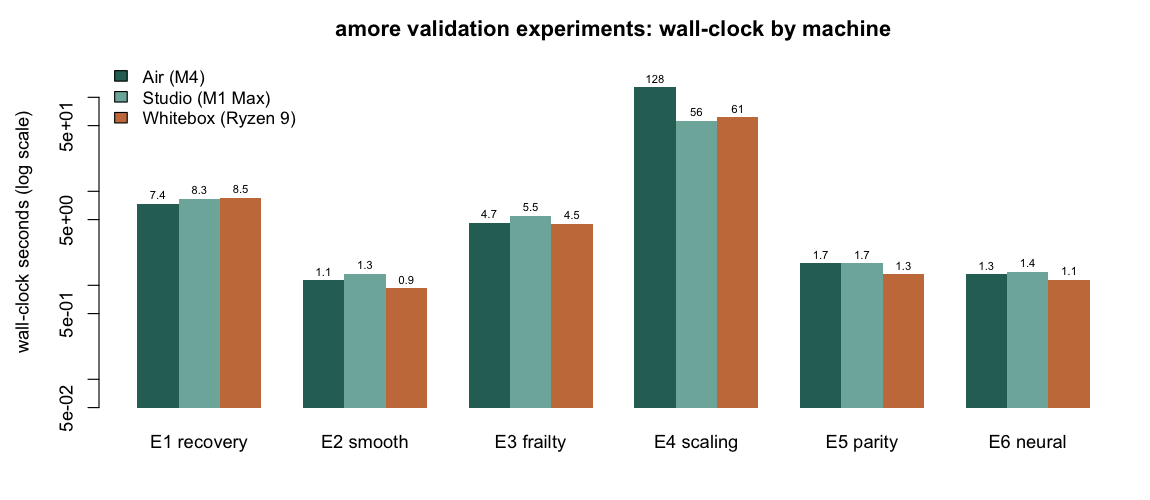
\includegraphics[width=\textwidth]{figs/benchmark-times.png}
\caption{Wall-clock per experiment and machine (log scale).}
\end{figure}

\section{Observations}

\begin{itemize}\itemsep3pt
  \item \textbf{Compute-bound experiments are close across a decade of
        silicon.} On the five compute-bound experiments (everything except
        E4) the three machines land within $\sim$25\% of each other. The M4
        Air is fastest on the longer single-threaded simulate-and-fit loops
        (E1: 7.4\,s vs 8.3/8.5\,s; E3: 4.7\,s vs 5.5\,s Studio), while the
        Ryzen workstation takes the short experiments (E2: 0.9\,s; E5:
        1.3\,s; E6: 1.1\,s) — consistent with a workload dominated by
        single-thread R evaluation and short C++ bursts, where none of the
        machines can use its core count.
  \item \textbf{E4 inverts the ranking, and the reason is memory, not
        CPU.} The scaling experiment deliberately includes $\tau$-leap
        divergence cells that allocate up to the 16\,GB vector cap. On the
        16\,GB Air those allocations compete with the OS and interactive
        session, and E4 takes 128\,s; on the 64\,GB Studio and 91\,GB
        Whitebox the same cells are absorbed in RAM and E4 takes 56--61\,s
        — the two big-memory hosts more than halve the Air's time despite
        older (M1~Max) or differently-built (conda-forge) stacks.
  \item \textbf{Totals are an E4 story.} Summed wall-clock: Air 144\,s,
        Studio 75\,s, Whitebox 78\,s. The ``slowest'' machine on paper is
        the fastest on most individual experiments; aggregate rankings of
        this suite measure the memory subsystem more than the CPU.
  \item \textbf{Practical placement.} For the package's day-to-day
        development loop (tests, single experiments) any of the three is
        comfortable; for memory-hungry simulation sweeps the Studio or
        Whitebox are the right hosts, and the Whitebox's idle 16-core CPU
        is the obvious target if the experiment harness is ever
        parallelised across replicates.
  \item \textbf{Portability dividend.} Standing the benchmark up on the
        Linux host surfaced two real packaging lessons at zero cost: built
        macOS artifacts (\texttt{src/*.so}) must be excluded from
        source bundles (an ``invalid ELF header'' failure otherwise), and
        one experiment script loaded the package via \texttt{library()}
        rather than \texttt{load\_all()}, which only worked on machines
        with a stale installed copy. Both are now fixed in the bundle.
\end{itemize}

\section{Caveats}

\begin{itemize}\itemsep2pt
  \item Single pass per machine; small-experiment timings ($<2$\,s) carry
        subprocess start-up noise of a few hundred milliseconds.
  \item The Studio is a shared host and carried background load during the
        run; its timings are an upper bound.
  \item R versions and BLAS/toolchains differ across hosts (CRAN vs
        conda-forge builds); this benchmarks \emph{fleet machines as
        configured}, not isolated silicon.
  \item E4 wall-clock includes deliberately failing cells whose cost is
        memory-bound, not compute-bound; see Observations.
\end{itemize}

\section{Reproducibility}

The bundle lives at \texttt{paper/benchmark/} (this report,
\texttt{gen\_report.R}, timing CSVs under \texttt{data/}) and on the hosts at
\texttt{\char`~/amore-benchmark/bundle} (Whitebox),
\texttt{/Users/scl/pancho/amore-benchmark/bundle} (Studio). Each host runs:
\begin{center}
\texttt{R\_MAX\_VSIZE=16Gb Rscript bench.R . <machine>}
\end{center}

\end{document}
